\section{The Field of Play}\label{sec:field-of-play}

\subsection{Dimensions}
The field of play must be rectangular\removed{,
of nominal size 9000\,mm$\times$6000\,mm.} \added{and its nominal size will be different for each division, as follows:}

\begin{enumerate}
\item \added{\textbf{Division A} of nominal size 12000\,mm$\times$9000\,mm.}
\item \added{\textbf{Division B} of nominal size 9000\,mm$\times$6000\,mm.}
\end{enumerate} 

The exact field dimensions and the field markings at the venue may vary by up
to $\pm10\%$ in each linear dimension.

The dimensions include boundary lines.
Dimensions of the field, goals, and special field areas are in millimetres and
are shown in \autoref{fig:quad_size_field} \added{for division A and in \autoref{fig:double_size_field} for division B.}

\begin{figure}[ht] % ht = here / t = top / b = bottom
  \centering
  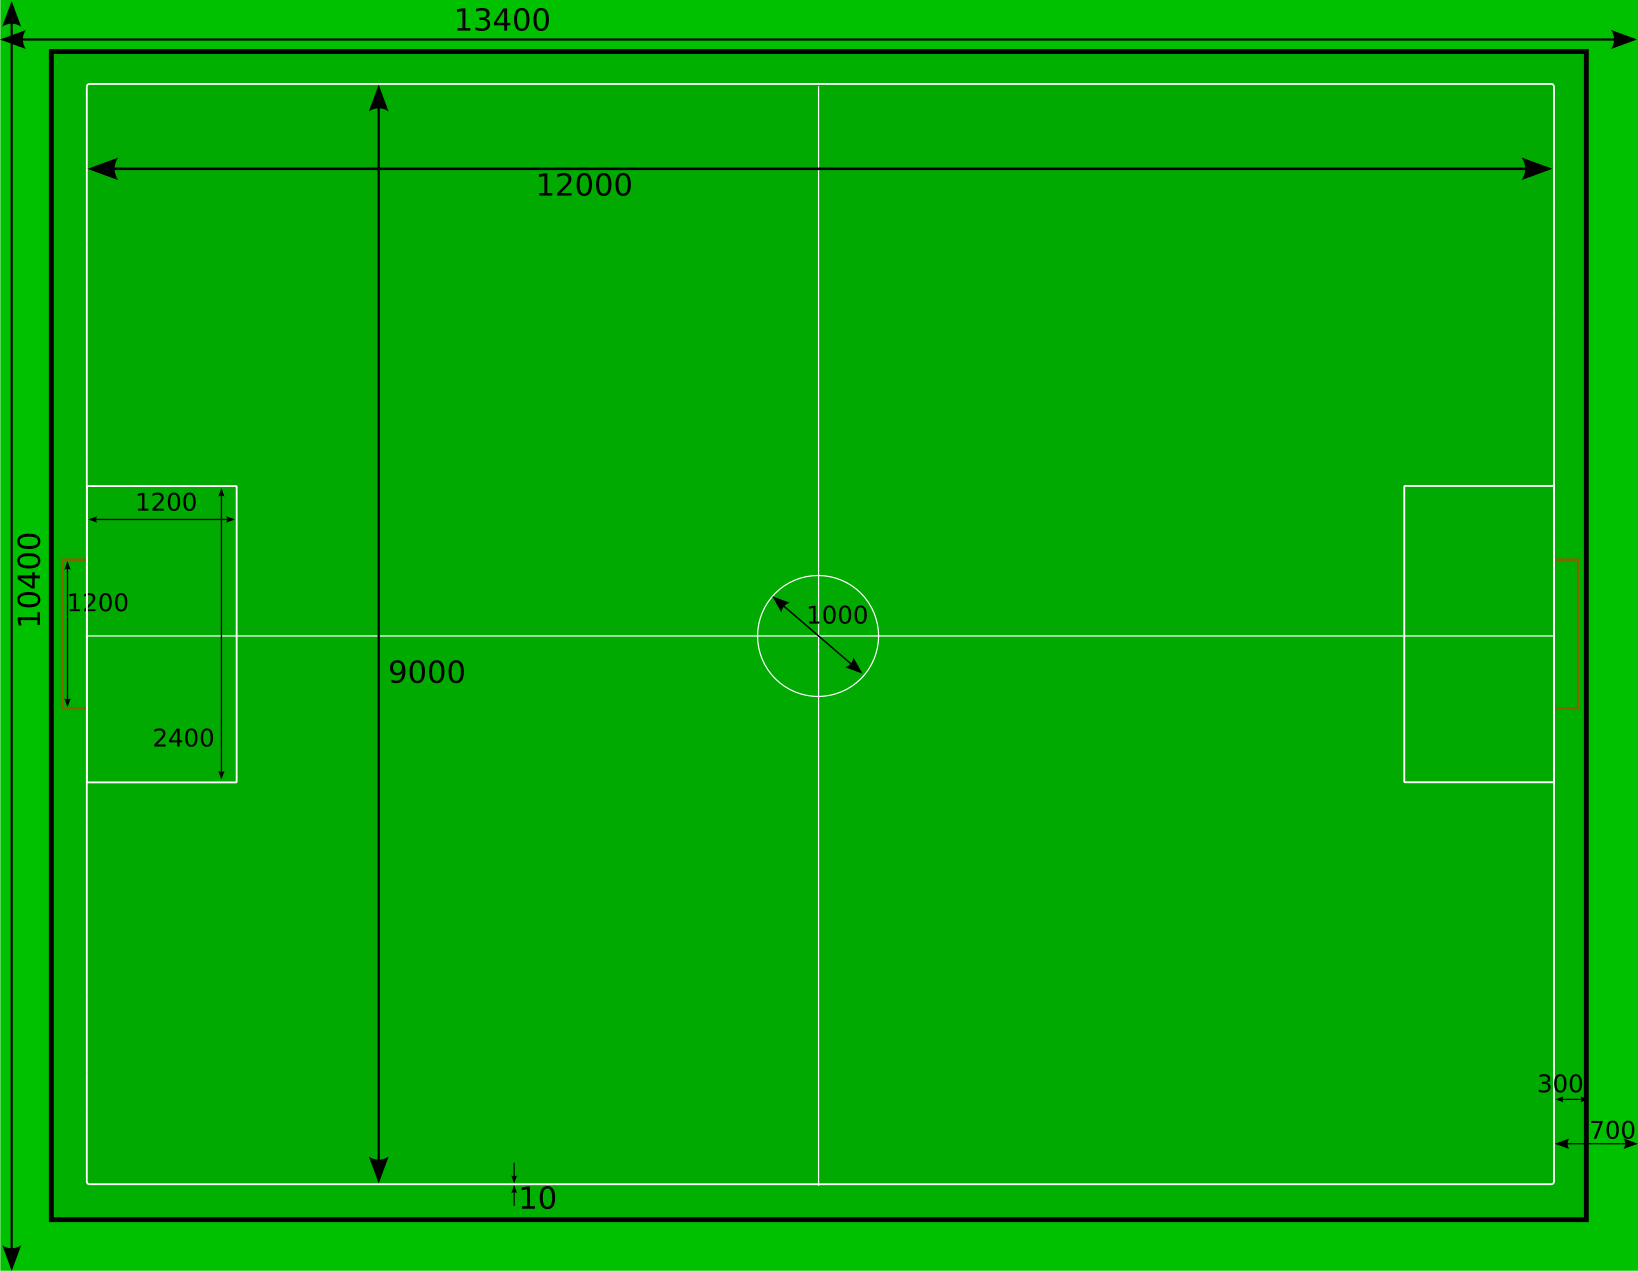
\includegraphics[width=0.8\columnwidth]{img/quad-size-field.png}
  \caption{\added{The field dimensions for division A}}
  \label{fig:quad_size_field}
\end{figure}

\begin{figure}[ht] % ht = here / t = top / b = bottom
  \centering
  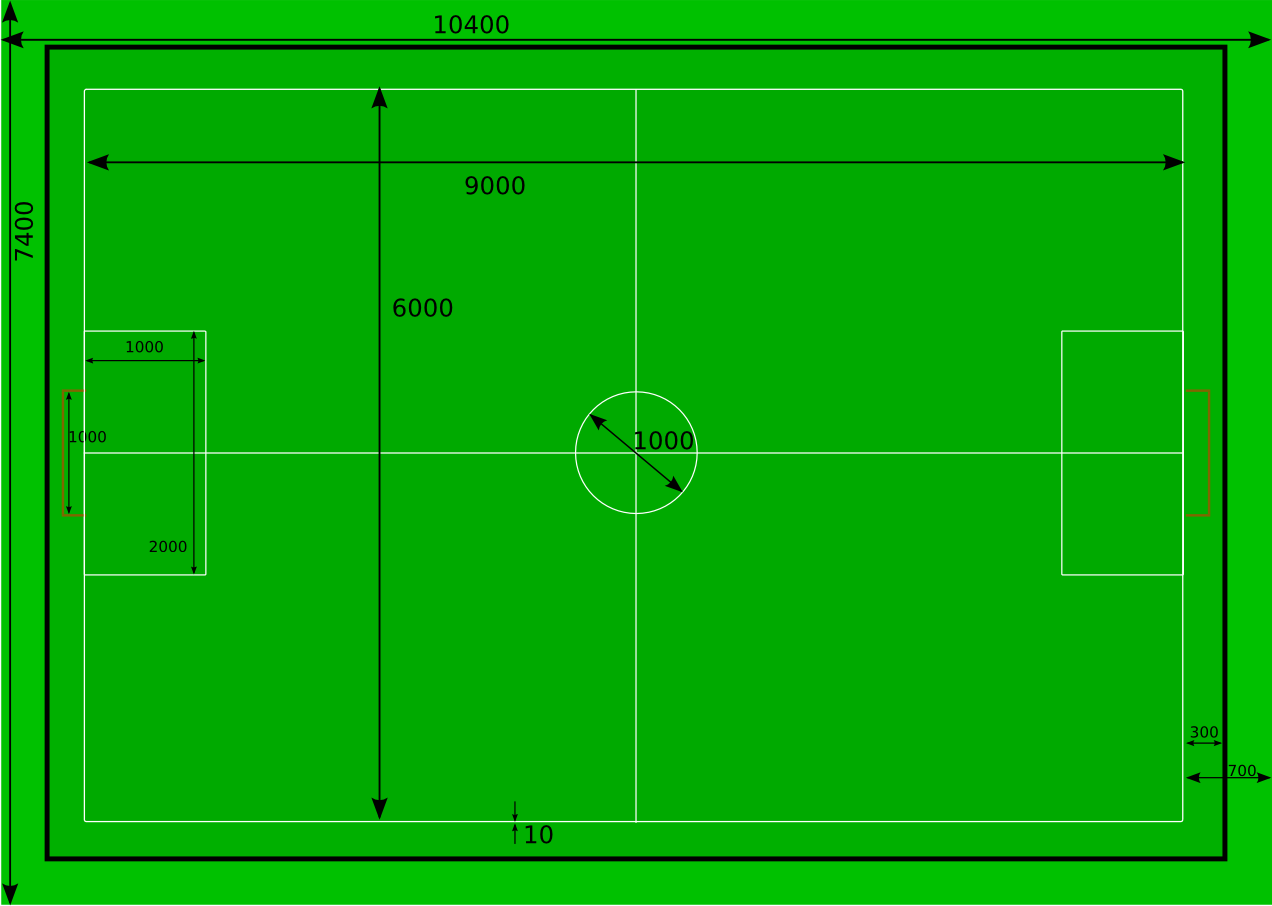
\includegraphics[width=0.8\columnwidth]{img/double-size-field.png}
  \caption{The field dimensions \added{for division B}}
  \label{fig:double_size_field}
\end{figure}

\subsection{Field Surface}
The playing surface is green felt mat or carpet.
The floor under the carpet is level, flat, and hard.

The field surface will continue for 700\,mm beyond
the boundary lines on all sides.
The outer 400\,mm of this runoff area, separated from the robot area by a
100\,mm tall wall, is used as a designated referee walking area (see
\autoref{sec:referee}).

\subsection{Field Markings}
The field of play is marked with lines.
Lines belong to the areas of which they are boundaries.

The two longer sides are called touch boundaries.
The two shorter sides are called goal boundaries.

All lines are 10\,mm wide and painted white.

The field of play is divided into two halves by a halfway line that runs
along the width of the field and through the center of the field.

A mid-line runs along the length of the field, passing through the center
  of the field. This line is used to provide adequate features for geometry
calibration of SSL-Vision.

The centre mark is indicated at the midpoint of the halfway line.
A  circle  with  a  diameter  of 1000\,mm is marked around it \added{for both divisions.}

\subsection{The Defence Area}

A defence area is defined at each end of the field as \added{a rectangle of 2400\,mm$\times$1200\,mm for division A and 2000\,mm$\times$1000\,mm for division B.}
\removed{follows:
Two quarter circles of radius of 1000\,mm
are drawn on the field of play. These quarter circles are connected by a line of
length 500\,mm parallel to the goal line.} \added{\autoref{fig:quad_size_field} and} Figure \ref{fig:double_size_field} \added{show}\removed{shows} this configuration.
The area bounded by \added{this rectangle} \removed{these arcs and the goal line}is
the defence area.


\subsection{Penalty Mark}

For each field half the penalty mark is 1200\,mm \added{for Division A and 1000\,mm for Division B}, from the midpoint between the goalposts and equidistant to them, thus coinciding with the outer edge of the defence area. The mark is a 10 mm diameter circle of white paint

\subsection{Goals}
Goals must be placed on the centre of each goal boundary and anchored
securely to the field surface.

They consist of two 160\,mm vertical side walls joined at the back by a 160\,mm
vertical rear wall. The inner face of the goal has to be covered with an energy
absorbing material such as foam to help absorb ball impacts and lessen the speed
of deflections.
The goal walls, edges, and tops are white in color.

\removed{There is a round steel cross bar that runs across the top of the goalmouth and
parallel to the goal line. It is no larger than 10\,mm in diameter, but is
sufficiently strong to deflect the ball. The bottom of the bar is 155\,mm from
the field surface, and the bar is dark in color to minimise interference with
vision systems.}The top of the goal is covered in a thin net to prevent the ball
from entering the goal from above. It is attached securely to the \removed{cross bar and}
goal walls.

The distance between the side walls is \added{1200\,mm for division A and} 1000\,mm\ \added{for division B}, and the goal is 180\,mm deep.
The goal walls are 20\,mm thick and touch the outer boundary of the field at
the goal line, but do not overlap or encroach on the field lines or the field. \added{\autoref{fig:sslgoal-divisionA} and \autoref{fig:sslgoal-divisionB} show these details for division A and division B respectively.}

The floor inside the goal is the same as the rest of the playing surface.

\begin{figure}[ht] % ht = here / t = top / b = bottom
  \centering
  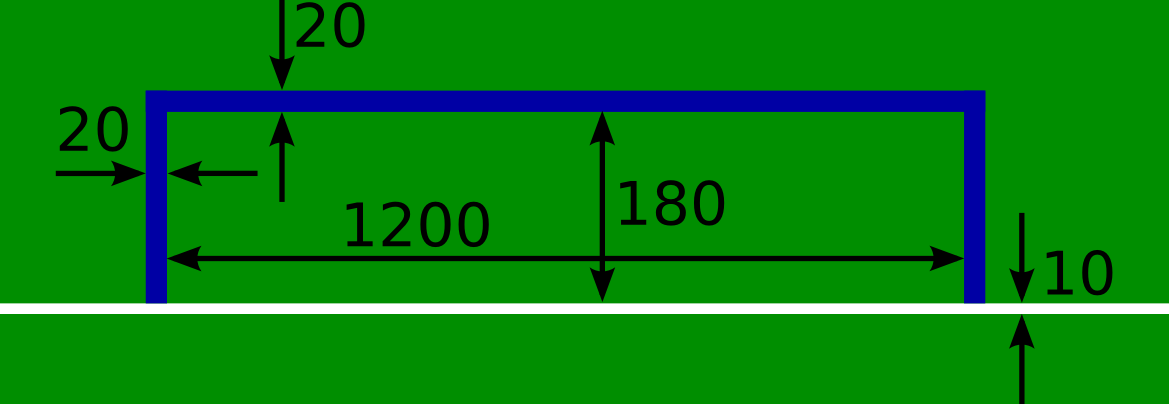
\includegraphics[width=0.5\columnwidth]{img/goal_detail_divisionA.png}
  \caption{\added{The Goal in detail for division A}}
  \label{fig:sslgoal-divisionA}
\end{figure}

\begin{figure}[ht] % ht = here / t = top / b = bottom
  \centering
  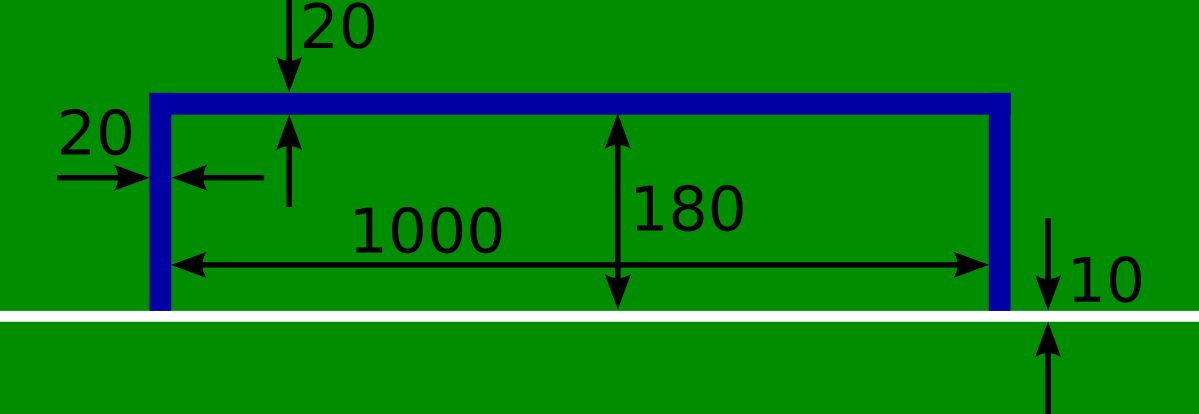
\includegraphics[width=0.5\columnwidth]{img/goal_detail_divisionB.png}
  \caption{The Goal in detail \added{for division B}}
  \label{fig:sslgoal-divisionB}
\end{figure}

\subsection{Equipment Mounting Bar}

A pair of mounting bars will be provided 4\,m
above the field. The bars will run parallel to the goal lines above the
center of each field half. The bars should be mounted
securely so that they do not swing or sway under a
small external force, and they should not bend or twist
significantly when the weight of typical video equipment is added.

\subsection{Shared Vision System}
Each field is provided with a shared central vision server and a set of shared
cameras. This shared vision equipment uses the community-maintained
\textbf{SSL-Vision}\footnote{\url{http://codegooglecom/p/ssl-vision/}} software
to provide localization data to teams via Ethernet in a packet format that is to
be announced by the shared vision system developers before the competition.
Teams need to ensure that their systems are compatible with the shared vision
system output and that their systems are able to handle the typical properties
of real-world sensory data as provided by the shared vision system (including
noise, latency, or occasional failed detections and misclassifications).
The vision patterns on the top of the robots must adhere to the
specifications of SSL-Vision, and must be of the standard color paper as
specified in the SSL-Vision documentation.

Besides the shared vision equipment, teams are \emph{not} allowed to mount
their own cameras or other external sensors, unless specifically announced or
permitted by the respective competition organisers.

The shared vision system in each field is maintained by one or more vision
experts. The procedure of selection of these experts will be announced by the
competition organisers. \autoref{app:vision-experts} describes the duties of the
vision experts.

\subsection*{Decisions of the Small Size League Technical Committee}
\begin{enumerate}
\item
The local organising committee should aim to provide uniform, diffuse lighting
conditions of approximately 500\,lux or brighter. No special lighting equipment
will necessarily be used to provide these conditions. The brightness is not
guaranteed nor expected to be fully uniform across the field surface. Teams are
thus expected to cope with the variations that will occur when using ambient
lighting. The organising committee will release details of the lighting
arrangements to the competitors as early as practical.

\item
No kind of commercial advertising, whether real or virtual, is permitted on the
field of play and field equipment (including the goal nets and the areas they
enclose) from the time the teams enter the field of play until they have left it
at half-time and from the time the teams re-enter the field of play until the
end of the match. In particular, no advertising material of any kind may be
displayed inside the goals or walls. No extraneous equipment (cameras,
microphones, etc.) may be attached to these items.

\item
The specific color and texture of the surface is not specified and may vary
from competition to competition (just as real soccer fields vary).
The surface underneath the carpet will be level and hard.
Examples of approved surfaces include: cement, linoleum, hardwood flooring,
plywood, ping-pong tables and particle board; carpeted or cushioned surfaces are
not allowed. Every effort shall be made to ensure that the surface is flat;
however, it is up to individual teams to design their robots to cope with slight
curvatures of the surface.
\end{enumerate}